\documentclass[UTF8,a4paper,11pt]{ctexart}

% ----- 宏包加载 -----
\usepackage[margin=2.5cm]{geometry}
\usepackage{amsmath, amsfonts, amssymb}
\usepackage{graphicx}
\usepackage{booktabs}
\usepackage{longtable}
\usepackage{array}
\usepackage{xcolor}
\usepackage{listings}
\usepackage{hyperref}
\usepackage{tikz}
\usepackage{float}
\usepackage{caption}
\usepackage{fancyhdr}
\usepackage{titlesec}
\usepackage[most]{tcolorbox}
\usetikzlibrary{shapes,arrows,positioning,fit,calc,shadows,backgrounds}

% ----- 颜色 -----
\definecolor{mainblue}{RGB}{0,70,127}
\definecolor{codegreen}{rgb}{0,0.6,0}
\definecolor{codegray}{rgb}{0.5,0.5,0.5}
\definecolor{codepurple}{rgb}{0.58,0,0.82}
\definecolor{backcolour}{rgb}{0.98,0.98,0.95}
\definecolor{warnred}{RGB}{180,40,40}

% ----- 代码风格 -----
\lstset{
    language=SQL,
    backgroundcolor=\color{backcolour},   
    commentstyle=\color{codegreen},
    keywordstyle=\color{mainblue}\bfseries,
    numberstyle=\tiny\color{codegray},
    stringstyle=\color{codepurple},
    basicstyle=\ttfamily\small,
    breaklines=true,                 
    numbers=left,                    
    numbersep=5pt,                  
    frame=leftline,
    rulecolor=\color{mainblue}
}

% ----- 页眉页脚 -----
\pagestyle{fancy}
\fancyhf{}
\lhead{\small AEDS 项目质量评估}
\rhead{\small \thepage}
\renewcommand{\headrulewidth}{0.5pt}

% ----- 标题样式 -----
\titleformat{\section}{\Large\bfseries\color{mainblue}}{\thesection}{1em}{}[\titlerule]

\begin{document}

\begin{center}
    {\LARGE \bfseries 翼型工程数据库系统 (AEDS)} \\
    \vspace{0.3cm}
    {\Large \textcolor{mainblue}{项目不足与缺点分析报告}} \\
    \vspace{0.2cm}
    {\normalsize —— 基于数据库原理与实践课程考核要求的系统复盘} \\
    \vspace{0.5cm}
    {\normalsize 评估日期：2026年6月21日}
\end{center}

\vspace{1cm}

\begin{tcolorbox}[colback=mainblue!5, colframe=mainblue, title=评估说明]
本报告以数据库原理与实践课程的大二软件工程专业学生视角，依据课程核心知识点（数据库设计、事务处理、并发控制、数据完整性、存储优化、SQL 查询性能、数据库安全性、系统开发），对 AEDS 项目的实现质量进行全面复盘。分析聚焦于项目在核心数据库理论落地过程中暴露出的设计缺陷与工程短板，不重复罗列已达标部分。
\end{tcolorbox}

\section{项目整体完成情况总评}

在正式进入不足分析之前，有必要客观评价项目的整体完成度。根据《差异检测报告（第 5 版）》的逐项对照，AEDS 系统在 35 项考核指标中实现了 \textbf{28 项完全达标 + 3 项部分达标}，综合达标率 \textbf{80\%}。具体而言：

\begin{itemize}
    \item \textbf{§5 系统功能要求}：7/7 项全部达标，CRUD、版本管理、坐标录入、性能录入均已通过 Web 交互实现闭环。
    \item \textbf{§7 高级机制实验}：索引优化（5.3x 性能提升）、事务并发（原子回滚 + 乐观锁/悲观锁）、视图/触发器/存储过程均已完成，21/21 项覆盖率检查 100\%。
    \item \textbf{§8 数据治理}：8 条异常检测规则 + 版本追溯 + 来源标记 + 软删除策略均已实现。
    \item \textbf{§10 可视化}：13 张 ECharts 图表 + 6 张 Matplotlib 静态图，远超文档要求的"两项以上"。
\end{itemize}

\textbf{然而}，在高达标率的表象下，项目中存在若干触及数据库课程核心考核维度的系统性短板。以下三点不足并非表层缺陷，而是从数据库原理的底层视角审视项目时必然浮现的实质性问题。

\section{不足一：事务原子性在业务层的落地断层}

\subsection{问题描述}

项目在 TestLab 实验套件中出色地验证了事务的原子回滚与并发隔离机制（见 \texttt{02\_transaction\_experiment.sql}），但在实际的 Web 业务代码中，事务管理呈现严重的"\textbf{实验与生产脱节}"现象。

\subsection{技术证据}

Django Webfront 的 DAO 层代码中，涉及\textbf{多表联合写入}的关键操作未使用显式事务包裹。以 \texttt{airfoil\_dao.py} 中的 \texttt{create\_airfoil()} 为例：

\begin{lstlisting}[caption=多表写入未包裹事务（airfoil\_dao.py）]
def create_airfoil(code, name, ...):
    with connection.cursor() as cursor:      # ← 仅管理游标生命周期
        # 写入 1: data_source
        cursor.execute("INSERT INTO data_source (...) VALUES (...)")
        # 写入 2: airfoil
        cursor.execute("INSERT INTO airfoil (...) VALUES (...)")
        # 写入 3: airfoil_version
        cursor.execute("INSERT INTO airfoil_version (...) VALUES (...)")
\end{lstlisting}

该函数使用 \texttt{with connection.cursor()} 上下文管理器，但\textbf{Django 的 cursor 上下文仅管理游标（cursor）的开闭，不提供事务管理语义}。在当前 Django 配置下（\texttt{ATOMIC\_REQUESTS=False}，即默认值），每个 \texttt{cursor.execute()} 在 autocommit 模式下独立提交。这意味着：
\begin{itemize}
    \item 若 \texttt{airfoil} 的 INSERT 成功但 \texttt{airfoil\_version} 的 INSERT 失败（如版本号冲突），\texttt{data\_source} 记录将成为孤儿数据（orphan record）。
    \item 系统失去了"要么三表同时写入，要么全部不写入"的原子性保证。
\end{itemize}

在整个 Webfront 代码库中，仅 \texttt{anomaly\_engine.py} 的批量扫描函数使用了 \texttt{transaction.atomic()}，而存在多表写入风险的操作（新建翼型、新建版本、新建性能数据——均涉及后台多 \texttt{INSERT} 步骤）全部依赖数据库的 autocommit 机制。

\subsection{课程知识映射}

数据库原理课程的"\textbf{事务}"一章明确指出事务的 ACID 属性是数据库区别于文件系统的核心特征。特别是\textbf{原子性（Atomicity）}要求：一个事务中的所有操作要么全部完成，要么全部不执行。当前系统的实现方式使得这一点在理论上被 TestLab 验证、在实际上被生产代码绕过，构成典型的"知识点掌握不完整"问题。

\subsection{修复思路}

在 \texttt{create\_airfoil}、\texttt{create\_version}、\texttt{add\_performance\_record} 等涉及多表写入的 DAO 函数中，添加 \texttt{with transaction.atomic():} 包装整个写入逻辑块。

\section{不足二：完整性约束设计的策略性妥协}

\subsection{问题描述}

项目在物理层 CHECK 约束的设计上存在一个值得从数据库原理角度深入审视的\textbf{构造性缺陷}：将业务语义标记（\texttt{is\_anomaly}）作为数据完整性约束的"豁免条件"，导致约束不再是绝对不可违反的物理规则。

\subsection{技术证据}

\texttt{performance\_record} 表上 Cd 约束的实际定义（见 \texttt{02\_constraints.sql}）：

\begin{lstlisting}[caption=条件化 CHECK 约束（02\_constraints.sql）]
ALTER TABLE public.performance_record
  ADD CONSTRAINT ck_performance_record_cd_or_anomaly
  CHECK (cd >= 0 OR is_anomaly);
\end{lstlisting}

该约束的逻辑语义是："Cd 必须大于等于 0，\textbf{除非}该记录被标记为异常"。这在工程上是务实的——它允许异常检测引擎将识别到的负 Cd 记录标注为异常而非直接拒绝写入。但从数据库原理的角度审视：

\begin{enumerate}
    \item \textbf{约束不再是约束}：\texttt{CHECK} 的原始设计意图是"物理不可违反"，而此处的 \texttt{is\_anomaly} 参数使得\texttt{任何能够设置 is\_anomaly=true 的应用程序}都可以绕过物理层的 Cd 约束。约束的执行权从 DBMS 转移到了应用层。
    \item \textbf{语义混乱}：\texttt{is\_anomaly} 是一个业务元数据标记（"这条数据疑似有问题"），却被用作物理约束的豁免条件（"因为标注了异常，所以允许违反物理定律"）。这两层语义的目的不同，强行耦合引入了概念上的自相矛盾。
    \item \textbf{课程标准对照}：文档 §6.3 明确要求 "\textbf{阻力系数 Cd 必须大于等于 0}"。当前实现添加了 \texttt{OR is\_anomaly} 后缀，严格来说只能算"Cd 大于等于 0 或被标记异常"，未完全满足文档的本意。
\end{enumerate}

此外，\texttt{experiment\_condition} 表缺少 (\texttt{alpha\_deg}, \texttt{reynolds\_number}) 的唯一性约束，理论上允许同一工况组合在表中以不同 UUID 重复出现。虽然 \texttt{performance\_record} 的联合唯一约束 (\texttt{version\_id}, \texttt{condition\_id}) 能间接避免重复性能记录，但物理层面没有防止工况参数表自身的冗余。

\subsection{课程知识映射}

数据库原理课程的"\textbf{完整性}"一章将约束分为实体完整性、参照完整性、用户定义完整性三类。\texttt{CHECK} 属于用户定义完整性，其设计原则是：\textbf{约束应在数据库层强制执行，不应依赖应用层的"自觉"}。当约束条件中引入可由应用层修改的字段作为豁免条件时，约束的物理强制性已经退化。

\subsection{修复思路}

\begin{itemize}
    \item 将 Cd 约束恢复为纯物理约束 \texttt{CHECK (cd >= 0)}，异常数据改为在应用层通过插入前校验捕获——\textbf{不让不合规数据落入数据库}，而非先写入再标记异常。
    \item 补充 \texttt{experiment\_condition} 表上的 \texttt{UNIQUE (alpha\_deg, reynolds\_number)} 约束。
\end{itemize}

\section{不足三：数据库安全性与访问控制的体系性缺失}

\subsection{问题描述}

文档 §6.1 要求至少包含 \texttt{User}（用户或操作人员）实体，项目在表结构上实现了 \texttt{user\_account} 表并建立了外键关联。但从\textbf{数据库安全性}这一课程核心知识点的视角审视，系统在访问控制、身份认证和权限管理方面存在系统性空白。

\subsection{技术证据}

\begin{enumerate}
    \item \textbf{表设计层面}：\texttt{user\_account} 表仅包含 \texttt{username} 和 \texttt{role} 两个字段，\textbf{缺少 \texttt{password\_hash}}——这意味着表中存储的是裸标识而非可认证的凭据。外键引用（如 \texttt{airfoil\_version.created\_by → user\_account.user\_id}）更多地起到"操作人记录"作用而非"访问控制"作用（见表 \ref{tab:user_table}）。
    
    \begin{table}[H]
    \centering
    \caption{\texttt{user\_account} 表结构分析}
    \label{tab:user_table}
    \begin{tabular}{lll}
    \toprule
    字段 & 类型 & 评估 \\
    \midrule
    \texttt{user\_id} & UUID PK & 符合规范 \\
    \texttt{username} & TEXT & 基本标识 \\
    \texttt{role} & TEXT & 枚举值未约束，无 CHECK \\
    \texttt{is\_active} & BOOLEAN & 有标记字段 \\
    \texttt{password\_hash} & \textbf{缺失} & \textbf{无法实现认证} \\
    \bottomrule
    \end{tabular}
    \end{table}

    \item \textbf{数据库层缺失}：系统未实现任何以下 PostgreSQL 数据库安全机制：
    \begin{itemize}
        \item \textbf{角色（Role）分离}：应用使用单一数据库连接用户，无法区分读写权限。
        \item \textbf{行级安全（RLS, Row-Level Security）}：未针对 \texttt{user\_account} 或敏感表启用 RLS 策略，所有用户可读取所有数据。
        \item \textbf{授权（GRANT / REVOKE）管理}：未在初始化脚本中建立按角色的表级权限分配。
    \end{itemize}

    \item \textbf{应用层退化}：Django Web 前端\textbf{主动移除了登录认证}（注释掉 \texttt{LOGIN\_URL}，禁用 \texttt{@login\_required} 装饰器），以追求"开箱即用"的易用性。这一设计选择在工程上可以理解（便于演示），但在课程考核的"数据库安全性"维度上构成实质性空白。
    
    \item \textbf{审计日志的伪安全性}：触发器 \texttt{trg\_log\_change\_*} 通过 \texttt{current\_setting('app.current\_user\_id')} 记录操作人，但\texttt{current\_setting} 是会话级变量，可由任意会话通过 \texttt{SET app.current\_user\_id = 'xxx'} 的方式伪造。它提供了可追溯性（auditability），但\textbf{不提供任何访问控制执行能力}（access control enforcement）。
\end{enumerate}

\subsection{课程知识映射}

数据库原理课程的"\textbf{安全性}"专题涵盖：身份认证（Authentication）、授权控制（Authorization）、强制访问控制（MAC）、自主访问控制（DAC）、审计追踪（Audit）。当前系统的 user\_account 表仅覆盖了审计追踪的"事后记录"层面，而完全缺失身份认证（无密码）和授权控制（无角色权限分级、无 RLS、无 GRANT/REVOKE）这两个更基本的数据库安全维度。

\subsection{修复思路}

\begin{itemize}
    \item \textbf{最低要求}：为 \texttt{user\_account} 表增加 \texttt{password\_hash}（至少使用 \texttt{pgcrypto} 扩展的 bcrypt 哈希），在应用层实现基于会话的登录认证。
    \item \textbf{课程合规}：建立至少两种数据库角色（\texttt{reader} / \texttt{editor}），使用 \texttt{GRANT SELECT}/\texttt{GRANT INSERT} 等语句分配表级权限。
    \item \textbf{进阶}：对性能数据等核心表启用 RLS 策略，基于 \texttt{created\_by} 字段限制用户只能修改自己创建的数据。
\end{itemize}

\section{系统性短板架构分析图}

\begin{figure}[H]
    \centering
    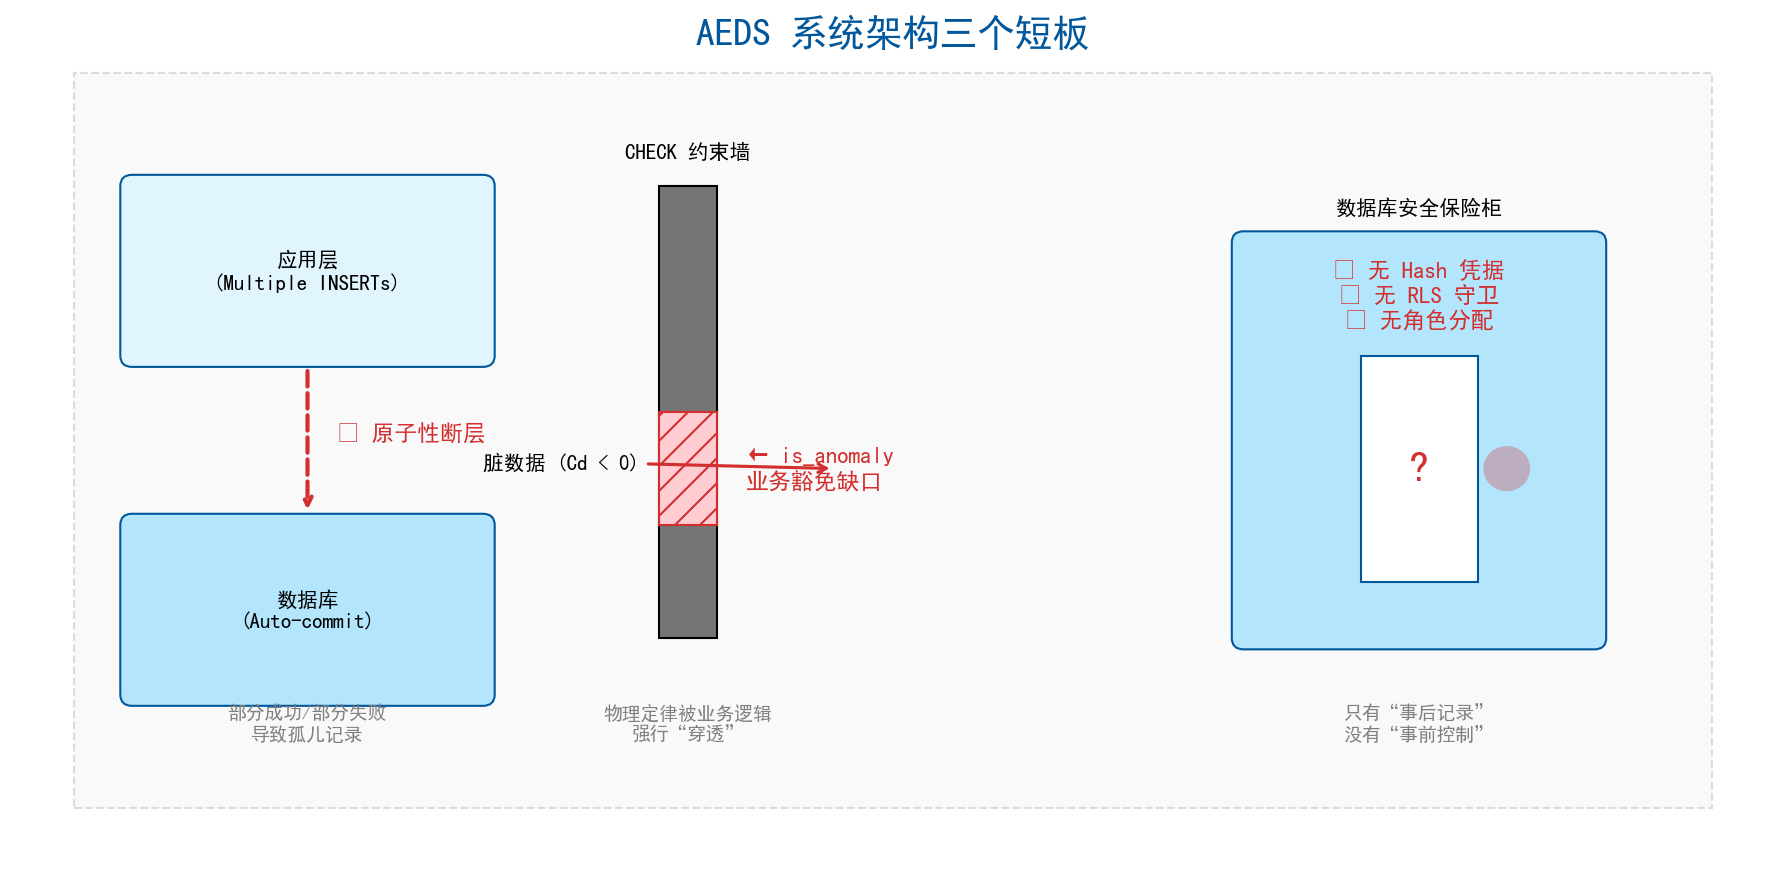
\includegraphics[width=\textwidth]{weakness_story.png}
    \caption{AEDS 系统架构中的三个关键短板：故事化呈现}
    \label{fig:weakness_story}
\end{figure}

\section{总结与课程反思}

\begin{tcolorbox}[colback=mainblue!5, colframe=mainblue, title=三点不足的课程知识点对应]
\begin{center}
\begin{tabular}{lll}
\toprule
不足 & 涉及课程核心章节 & 问题性质 \\
\midrule
事务落地断层 & 事务处理 \& 并发控制 & 理论与实践脱节 \\
完整性约束妥协 & 数据完整性 \& 约束设计 & 设计选择有瑕疵 \\
安全性体系缺失 & 数据库安全性 & 核心维度系统性空白 \\
\bottomrule
\end{tabular}
\end{center}
\end{tcolorbox}

从大二学生的角度审视，AEDS 项目的工程完成度较高（80\% 达标率），Web 前端实现了丰富的交互功能，TestLab 实验套件覆盖了索引、事务和高级对象的全套验证。然而，数据库原理课程的考核核心并非"功能做得多的少"，而是"\textbf{数据库理论是否真正落地}"。以上三点不足共同揭示了一个深层问题：项目在"\textbf{把实验结论转化为生产代码}"这一环节存在断层——事务机制在 SQL 脚本中被验证了，但 Web 代码中没有用上；约束概念理解了，但设计时引入了业务层面的妥协；user 表建了，但安全性三个字始终停留在"做记录"而非"做控制"的层面。

这三点不足为后续版本改进提供了明确的技术锚点，也是数据库课程从"会用"到"会用对"这一关键跨越的真实写照。

\end{document}
